\apendice{Documentación de usuario}

\section{Introducción}
El usuario es aquella persona destinada a utilizar el Sistema generado.

\section{Requisitos de la instalación física}
Se incluye la instalación en este punto porque se entiende que cualquiera que disponga el código puede correrlo en su propia instalación realizando la instalación física.

\section{Instalación física}
Para poder realizar la instalación física de nuestra instalación necesitamos el material detallado en la tabla~\ref{tab:CosteHW}, ya que en este punto se cuenta con que la instalación física está completa para que el sistema pueda cumplir su cometido. Ahora utilizaremos los siguientes materiales:
\begin{itemize}
    \item Bobina de Cable UTP5e.
    \item Placa Board.
    \item Relés con las características: [ 10A 250VAC 10A 125VAC ]~[ 10A 30VDC 10A 28VDC ].
    \item Cables de electrónica.
    \item Conectores JST-XH.
\end{itemize}

Además requeriremos de crimpadora JST-XH y destornilladores de estrella y plano para trabajar con las clemas eléctricas (elementos de interconexión de conductores) del domicilio.

También necesitamos otros elementos de uso no específico para este proyecto pero que resultan necesarios para que el software funcione correctamente~\footnote{El software puede funcionar correctamente también vía Ethernet.} como son el Dongle Wifi y una línea de datos con salida a Internet.

\subsection{Tirada de cable}
Para realizar la tirada de cable necesitaremos hacer algunos cálculos y tener claras algunas consideraciones:

\subsubsection{Consideraciones}
Debemos tener claras las características eléctricas que soporta cada uno de los pines GPIO de nuestra Raspberry Pi. Cada uno de los pines, soporta 3,3VDC~\footnote{VDC:Voltage Direct Current.} y 16 mA, excepto algunos pines de alimentación, que cuentan con hasta 5VDC.
Hay que comprobar que cada uno de los hilos del cable UTP5e que vamos a instalar soporta la señal que vamos a transmitir por el cable aunque según la norma TIA/EIA568, en el punto A.3 especifica que deben pasar pruebas de hasta 500VDC y un mínimo entre dos cables de 100M\si{\ohm}. Además, también se especifica que debe contar con un AWG~\cite{wiki:DefAWG} de, entre 22 y 24, lo que se traduce en que soporta 0.577A-0.92A~\cite{wiki:TablaAWG}, respectivamente.

\subsubsection{Cálculos necesarios}
Debemos calcular si podemos introducir nuestros cables por los tubos con seguridad. Esto viene recogido en el REBT, más concretamente en apartado ITC\_BT\_21 de éste.

Sabiendo que nuestro cable UTP tiene unos 5mm de diámetro de sección, que la cara interna del tubo es de 17,8mm y que cada cable eléctrico tiene un área de 1,5mm$^{2}$ podemos calcular el área total ocupada y el tubo por el que debería hacerse la instalación con la seguridad requerida por norma:
\begin{equation}
\centering
\pi \cdot D^2/4 >= FactorCorrector \cdot (\sum(NumeroDeCabes \cdot \pi \cdot DiametroCable/4))
\end{equation}\label{E1}

Si realizamos el cálculo, observamos que la suma del área que ocupan los tres cables de 1,5mm$^{2}$ con el área del UTP (19,63mm$^{2}$) hace una ocupación total de 24,13mm$^{2}$.

Por otro lado, tenemos que el tubo que alberga los cables es de 20mm de diámetro de sección por la parte exterior del tubo y 17,80mm por la parte interna. Si calculamos el área interna obtenemos 248,85mm$^{2}$.
Según norma debemos ocupar la tercera parte del tubo. Para comprobar que el tubo puede contener los cables con seguridad, debemos calcular si la multiplicación del factor de corrección (en este caso de \textbf{3} por estar en una canalización empotrada de una vivienda), por la suma de las áreas que ocupan cada uno de los cables: 
\begin{equation}
\centering
3 \cdot [(3 \cdot 1,5)+(1 \cdot 19,63)]=72,40
\end{equation}\label{E2}

Ahora, debemos hacer el mismo cálculo del área de la cara interna del tubo:
\begin{equation}
\centering
\pi \cdot (17,8)/4
\end{equation}\label{E3}
Finalmente, vemos que~\ref{E3} es mayor que~\ref{E2} de forma que se cumple que el área ocupada (multiplicada por el factor de corrección) es inferior al área total, de modo que podemos albergar nuestro UTP en los tubos sin problema.

Por facilitar futuras instalaciones, figuro el cálculo para el mismo tubo también con cables de 2.5mm$^{2}$ de área en la imagen~\ref{Img:Calculo}:

\begin{figure}[h]
    \centering
    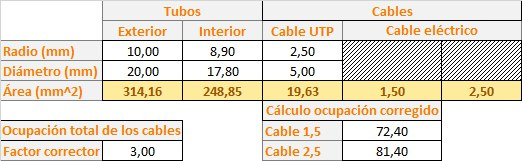
\includegraphics[width=0.9\textwidth]{img/Diagramas/calculo cables.jpeg}
    \caption{Cálculos para introducir cableado en tubo.} \label{Img:Calculo}
\end{figure}

Tras finalizar los cálculos, se hacen las tiradas de cableado y se crimpan los extremos. Podemos ver en la imagen~\ref{Img:CajaDerivacion} una caja de derivación donde ya tenemos albergada la placa de relés.~\\~\\

\begin{figure}[h]
    \centering
    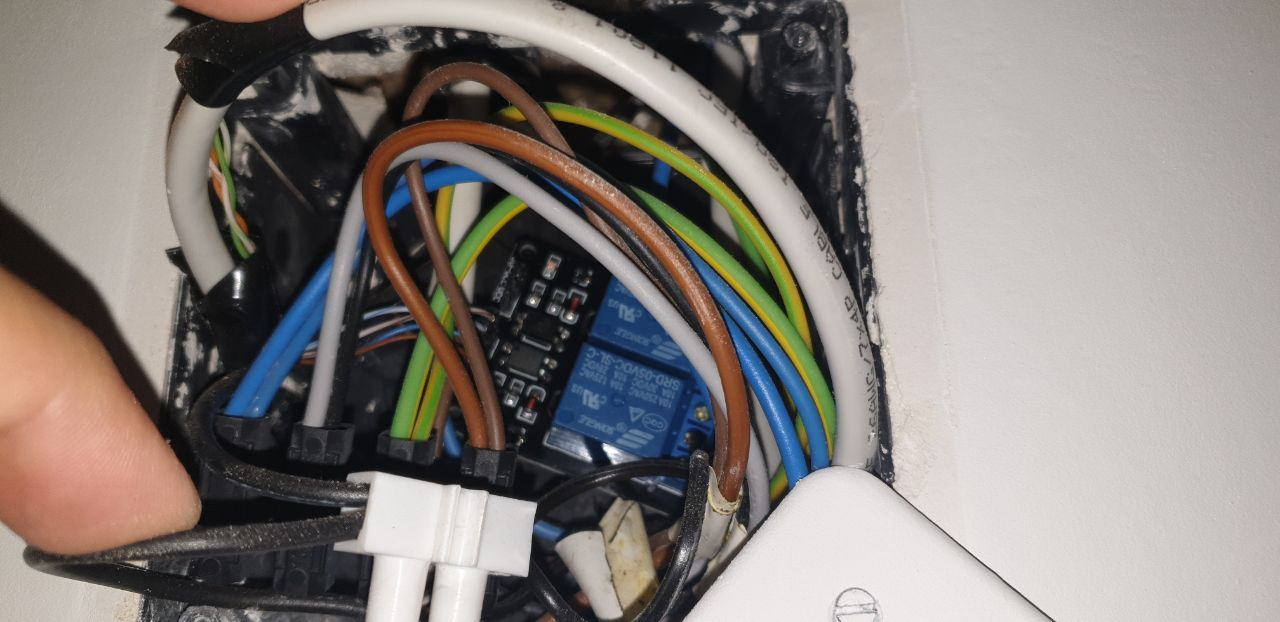
\includegraphics[width=0.9\textwidth]{img/fotos/caja-persiana.jpeg}
    \caption{Caja de derivación secundaria instalada.} \label{Img:CajaDerivacion}
\end{figure}

En la imagen~\ref{Img:CajaDerivacionPrincipal} vemos la caja de derivación principal con la instalación terminada indicando algunos elementos.

\begin{figure}[h]
    \centering
    \includegraphics[width=0.9\textwidth]{img/fotos/explicación caja instalada.jpg}
    \caption{Caja de derivación principal instalada.} \label{Img:CajaDerivacionPrincipal}
\end{figure}

El primer extremo del cable, podemos ver que termina en el relé dentro de la caja de derivación pero el extremo que conectará a la Raspberry Pi no se conectará directamente sino que terminará primero en una protoboard como podemos ver en la imagen~\ref{Img:ProtoboardConecada}, donde podemos diferenciar que existen dos tipos de conectores. Los redondos ya vienen conectorizados de fábrica pero los cuadrados del tipo~\href{https://ae01.alicdn.com/kf/H4205e9c4ec4c4be4864e44b6925a22bdf/10-juegos-de-conector-de-Cable-de-2-54mm-XH2-54-conector-XH-macho-y-hembra.jpg_Q90.jpg_.webp}{JST-XH} los he fabricado según las necesidades.~\\~\\

\begin{figure}[h]
    \centering
    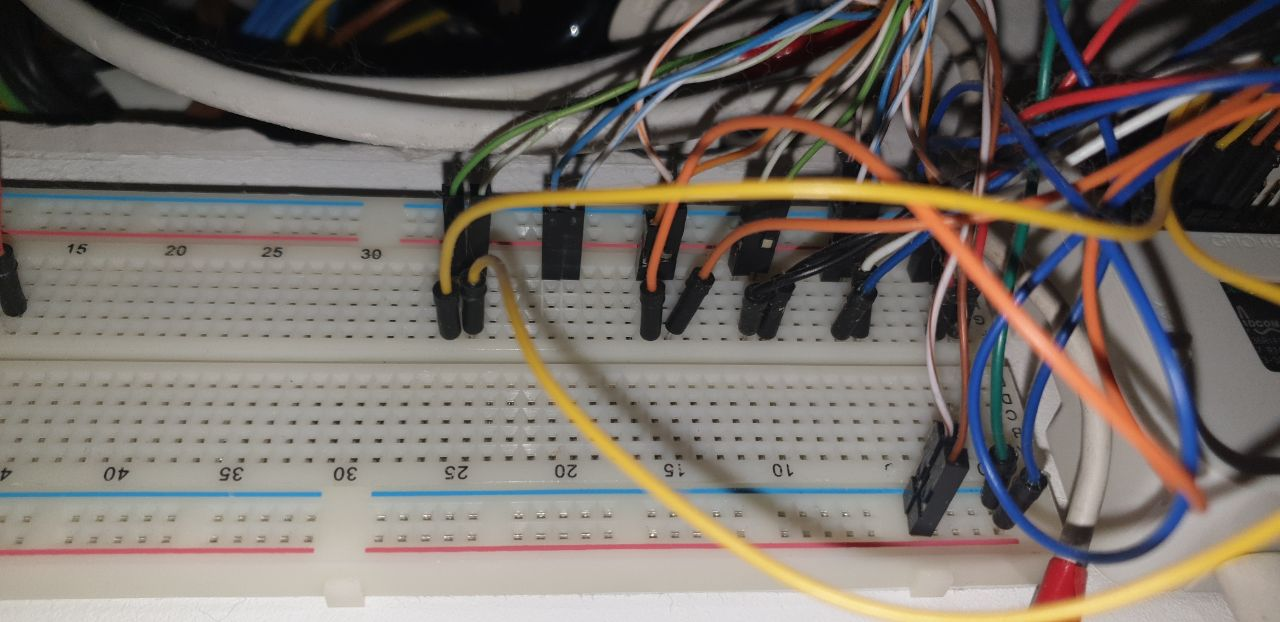
\includegraphics[width=0.7\textwidth]{img/fotos/protoboard-instalada.jpeg}
    \caption{Protoboard conectada.} \label{Img:ProtoboardConecada}
\end{figure}

En la imagen~\ref{Img:InstalacionDomotica} podemos ver la situación final de la tirada de cable y conectorizado.~\\~\\

\begin{figure}[h]
    \centering
    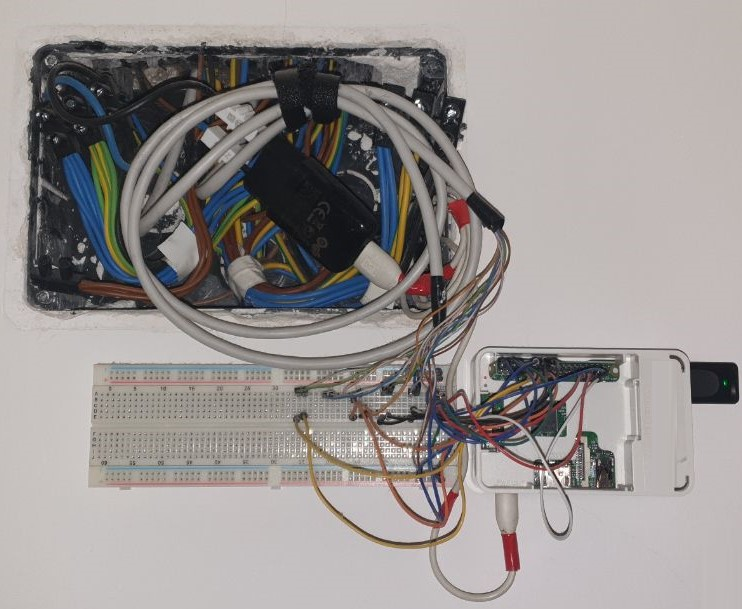
\includegraphics[width=0.9\textwidth]{img/fotos/RBP-instalada.jpeg}
    \caption{Instalación domótica y caja de derivación principal.} \label{Img:InstalacionDomotica}
\end{figure}


\begin{figure}[h]
    \centering
    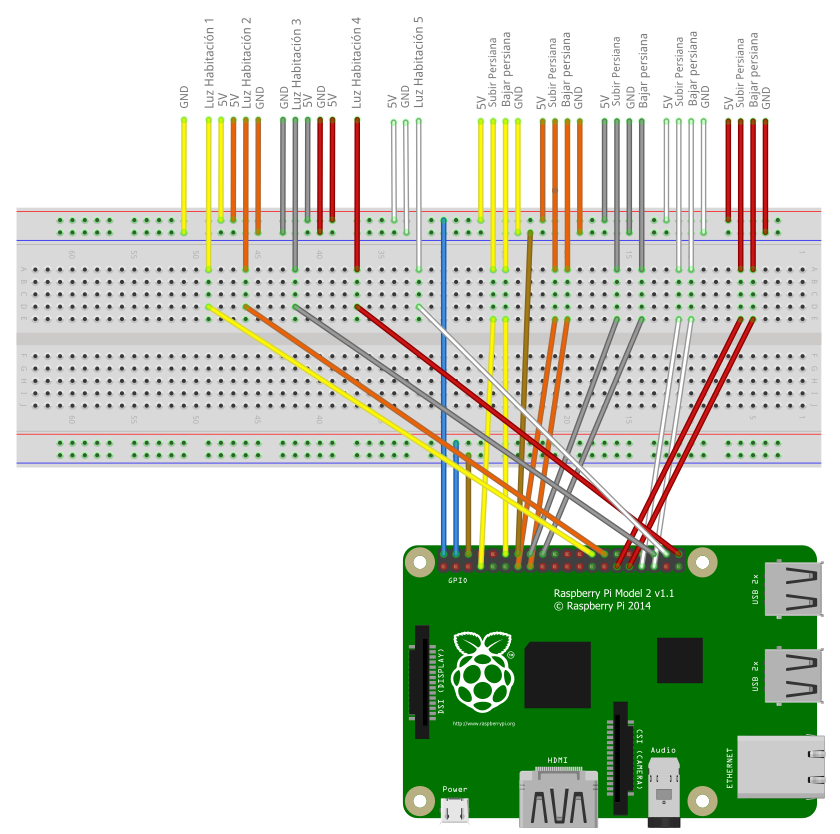
\includegraphics[width=0.9\textwidth]{img/RbP_CompletaLineas.png}
    \caption{Conectorizado final de las líneas GPIO.} \label{Img:RbP_CompletaLineas}
\end{figure}

El conectorizado final de las salidas de los GPIO es el que se puede ver en la imagen~\ref{Img:RbP_CompletaLineas}

Podemos interactuar con los puertos GPIO desde Bash y desde Python~\cite{misc:Python}. Se ha decidido utilizar lenguaje Bash para interactuar con los GPIO, dejando la potencia de Python para la obtención y procesado de datos. En ocasiones se producen errores al lanzar desde Cron scripts Python, por lo que se lanzará todo desde scripts bash.


\subsection{Diagramas eléctricos}
Para mayor claridad he generado unos planos eléctricos para aclarar como se ha realizado la instalación.

\begin{figure}[h]
    \centering
    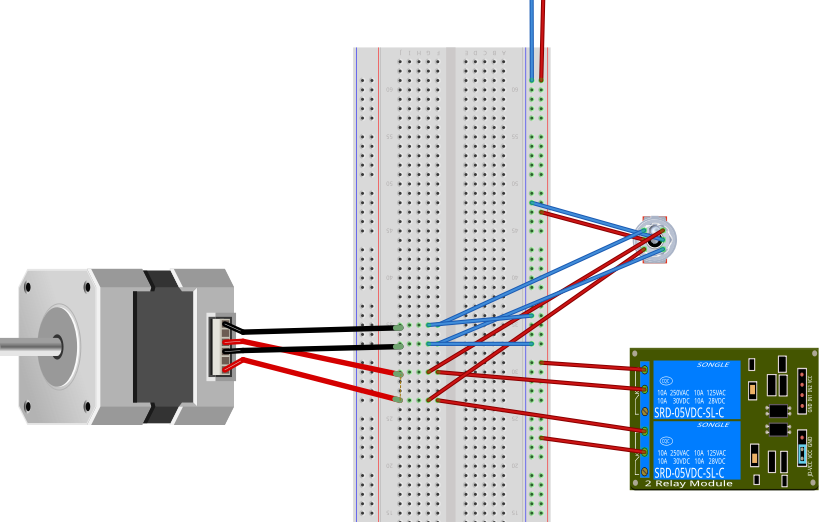
\includegraphics[width=0.9\textwidth]{img/Diagramas/rele-pulsador-motor.png}
    \caption{Raspberry Pi, relé y pulsador.} \label{Img:Relé+Pulsador+Rbp_Fritzing}
\end{figure}

En la imagen~\ref{Img:Relé+Pulsador+Rbp_Fritzing} podemos ver que tenemos conectada una placa con dos relés y un pulsador en paralelo, con el motor de la persiana. La protoboard realmente no existe en este punto pero la he incluido para clarificar el circuito.

En la imagen~\ref{Img:Relé+Rbp_Fritzing} podemos ver como se conecta, desde la Raspberry, el relé que conecta con una persiana identificando cada uno de los pines.

\begin{figure}[h]
    \centering
    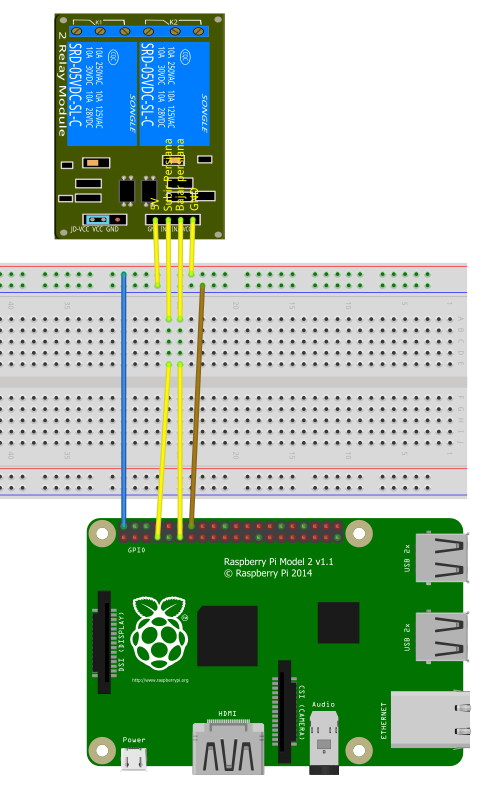
\includegraphics[width=0.5\textwidth, angle =90]{img/Diagramas/relé-RBP.png}
    \caption{Raspberry y relé conectados.} \label{Img:Relé+Rbp_Fritzing}
\end{figure}

\begin{figure}[h]
    \centering
    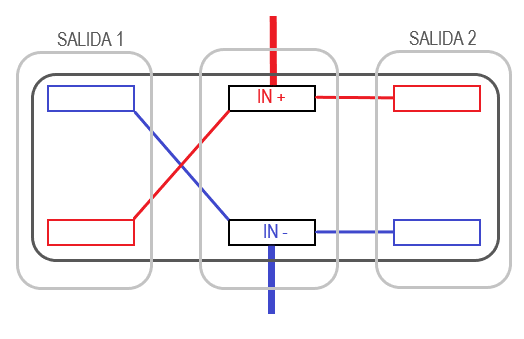
\includegraphics[width=0.6\textwidth]{img/Diagramas/PulsadorInterno.png}
    \caption{Funcionamiento interno de un pulsador para persianas.} \label{img:PulsadorInterno}
\end{figure}


Para explicar el funcionamiento de un pulsador de 3 posiciones para persianas podemos ver la imagen~\ref{img:PulsadorInterno}. En ella podemos ver como en la posición central no tiene ninguna salida, pero en la salida 1 el orden de salida de cabes es (+/-) y en la salida 2 el orden de salida de cables es (-/+). La lógica del cambio de orden en la salida de cables es porque según el sentido de la polaridad el motor girará en un sentido o en otro. Esto se respalda mediante la~\href{https://fisica.laguia2000.com/dinamica-clasica/fuerzas/ley-de-laplace-fuerza-ejercida-sobre-un-conductor}{segunda ley de Laplace} para cada espira del bobinado del motor quedando de la forma~\href{http://www.uco.es/grupos/giie/cirweb/teoria/tema_11/tema_11_01.pdf}{$M=N*(I*B*l+sen\theta)$}.

Siguiendo esta lógica, podemos ver que en la imagen~\ref{Img:Relé+Pulsador+Rbp_Fritzing} tenemos dos relés de forma que cada uno de ellos deja pasar la corriente en un sentido. En la realidad, el motor no tiene por qué tener dos entradas positivas y dos negativas pero en el dibujo queda mejor ilustrado que son entradas diferentes.

Resumiendo, la instalación mecánica y nuestra instalación mediante relés se instalarán en paralelo para poder activar una opción o la otra según la ocasión.

\section{Requisitos de usuarios}
Para poder ejecutar el código, el usuario necesitará este material, que también podemos ver en la imagen~\ref{material}:
\begin{itemize}
    \item Un terminal que soporte mensajería mediante Telegram. Cabe recordar que Telegram es multiplataforma, de modo que serviría un ordenador, un smartphone o un smartwatch entre otros.
    \item Una Raspberry Pi conectada a Internet.
    \item Una tarjeta uSD que haga de disco duro de nuestra Raspberry Pi.
    \item Alimentación de 2A para la Raspberry Pi.
    \item Otro equipo desde el que descargar y montar el Sistema Operativo de Raspberry Pi.
    \item Necesita generar cuentas en Climacell y WeatherAPI y un bot en BotFather.
\end{itemize}

\begin{figure}[!h]
\centering
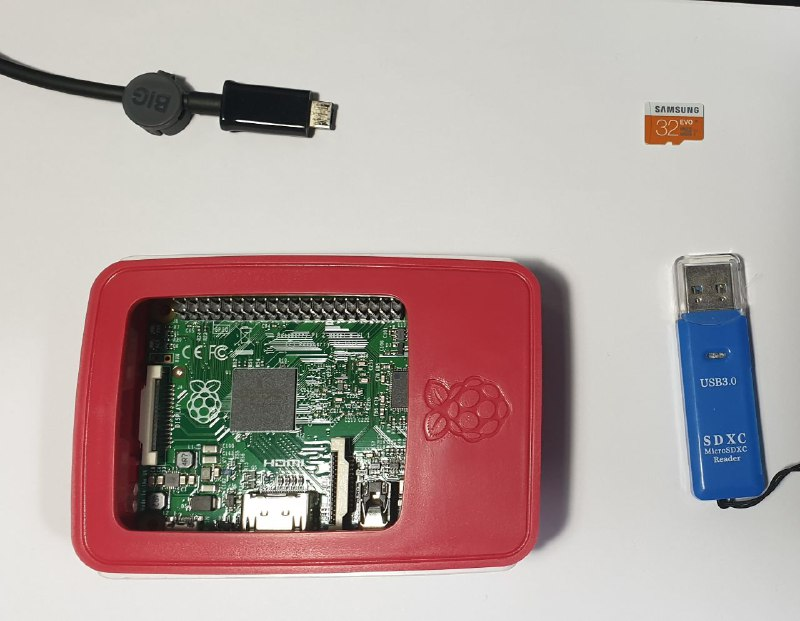
\includegraphics[width=0.7\textwidth]{img/fotos/RbP+SD+pen.jpeg}
\caption{Material básico para ejecutar el código.}\label{material}
\end{figure}

\section{Obtención de tokens}
En este punto se indica como obtener un token para poder utilizar las APIs.

\subsection{Climacell}
La primera API es Climacell. Para obtener el token debemos realizar los siguientes pasos:
\begin{itemize}
    \item Accedemos a la web oficial:~\url{https://www.climacell.co/pricing/}.
    \item Seleccionamos la opción gratuita.
    \item Rellenamos los datos que nos piden.
    \item Obtenemos el token de la pantalla que nos aparece.
\end{itemize}
Este token debemos guardarle muy bien puesto que es uno de los que utilizaremos para que el sistema funcione correctamente.

\subsection{WeatherApi}
La segunda API es WeatherApi. Para obtener el token debemos realizar los siguientes pasos:
\begin{itemize}
    \item Accedemos a la web oficial:~\url{https://openweathermap.org/price}.
    \item Seleccionamos la opción gratuita.
    \item Rellenamos los datos que nos piden.
    \item Accedemos a la pestaña de API Keys.
    \item Obtenemos el token de la pantalla que nos aparece.
\end{itemize}
Este token también debemos guardarle muy bien puesto que es uno de los que utilizaremos para que el sistema funcione correctamente.

\subsection{BotFather}
Los pasos para crear nuestro bot y obtener su token, son:
\begin{itemize}
    \item Desde una instancia logada de Telegram debemos buscar un chat llamado BotFather.
    \item Le enviamos el mensaje~\texttt{/start}
    \item Le enviamos el mensaje~\texttt{/newbot}
    \item Ahora, debemos enviarle el nombre que queremos ponerle a nuestro bot.
    \item La respuesta del BotFather es un mensaje donde nos indica el nombre de nuesto bot y el token que debemos guardar (en rojo).
\end{itemize}
Éste es el último token que debemos guardar para completar el archivo \texttt{config2.bot}.

\section{Instalación}

\subsection{Sistema Operativo}
El primer paso es descargar el Sistema Operativo de la web oficial y montarlo en la tarjeta SD con la ayuda de otro equipo informático y el adaptador USB para uSD que vemos en la imagen\label{material}. 

\begin{enumerate}
    \item Accedemos a: \url{https://www.raspberrypi.org/software/}
    \item Descargamos el software para montar la imagen en nuestra uSD \url{https://downloads.raspberrypi.org/imager/imager_1.5.exe}
    \item Introducimos el adaptador USB con la uSD en el equipo y corremos el software <<imagen\_1.5.exe>> para instalarlo, en este caso.
    \item En la ventana de instalación, seleccionamos <<install>> como figura en la imagen~\ref{instalacionRaspbian} para instalar el programa <<imager>> de Raspberry Pi Foundation.
\end{enumerate}

\begin{figure}[h]
\centering
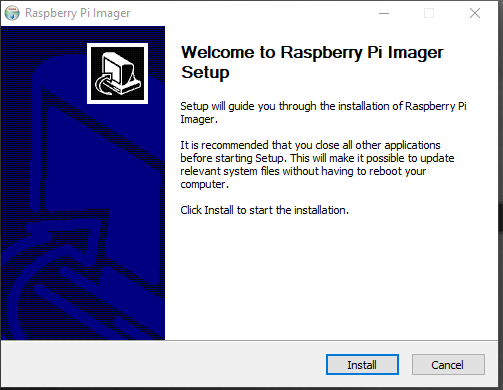
\includegraphics[width=0.7\textwidth]{img/fotos/instalacionRaspbian.PNG}
\caption{Ventana instalación <<imager>>, de Raspberry Foundation.}\label{instalacionRaspbian}
\end{figure}

\begin{enumerate}
\setcounter{enumi}{4}
    \item Seleccionamos las opciones de <<Sistema Operativo>> y <<SD Card>> como figura en la imagen~\ref{flasheadoSDRbP}.
\end{enumerate}

\begin{figure}[h]
\centering
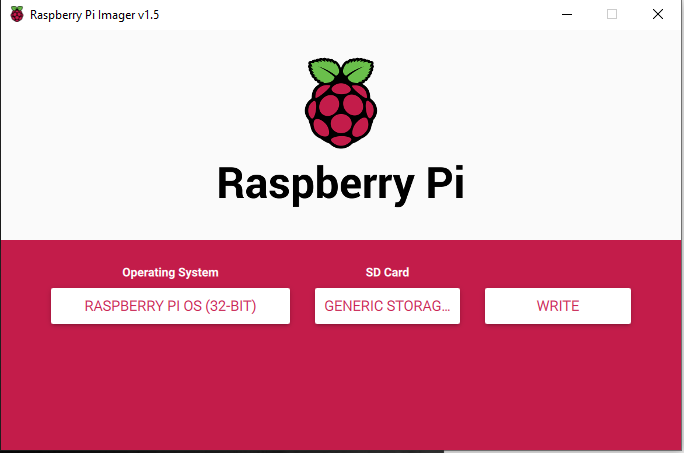
\includegraphics[width=0.8\textwidth]{img/fotos/flasheadoSDRbP.PNG}
\caption{Ventana selección imagen Raspbian.}\label{flasheadoSDRbP}
\end{figure}

\begin{enumerate}
\setcounter{enumi}{5}
    \item Una vez termine la grabación de la tarjeta, procederemos a introducirla en la Raspberry Pi por la ranura destinada a ello en la parte inferior de la placa y podremos acceder a Sistema Operativo con la ayuda de una pantalla, un teclado y un ratón.
    \item Debemos completar las siguientes ventanas de configuración:
\end{enumerate}

\begin{figure}[h]
\centering
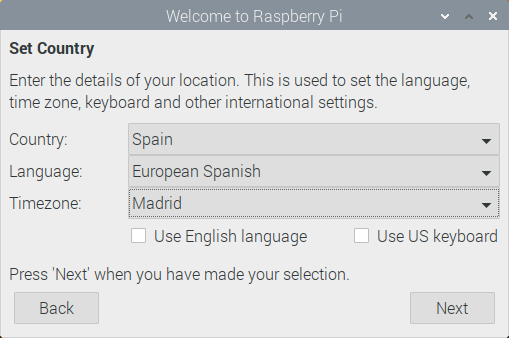
\includegraphics[width=0.8\textwidth]{img/Instalación/1.png}
\caption{Ventana de configuración Raspbian 1.}\label{Instala1}
\end{figure}

\begin{figure}[h]
\centering
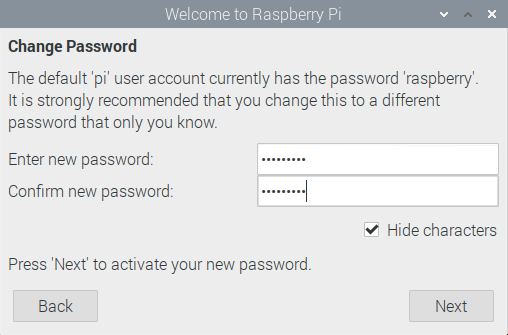
\includegraphics[width=0.8\textwidth]{img/Instalación/2.png}
\caption{Ventana de configuración Raspbian 2.}\label{Instala2}
\end{figure}

\begin{figure}[h]
\centering
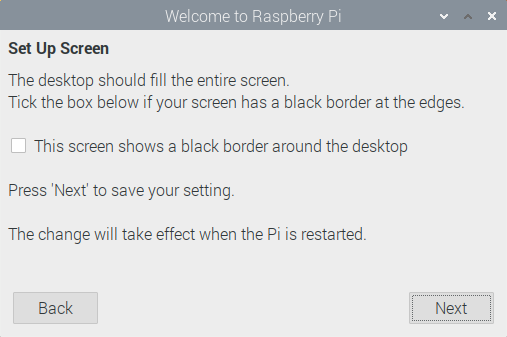
\includegraphics[width=0.8\textwidth]{img/Instalación/3.png}
\caption{Ventana de configuración Raspbian 3.}\label{Instala3}
\end{figure}

\begin{figure}[h]
\centering
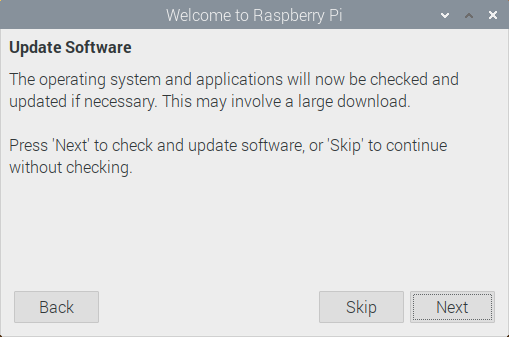
\includegraphics[width=0.8\textwidth]{img/Instalación/4.png}
\caption{Ventana de configuración Raspbian 4.}\label{Instala4}
\end{figure}

\begin{figure}[h]
\centering
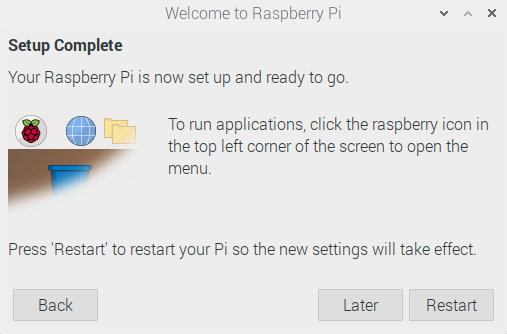
\includegraphics[width=0.8\textwidth]{img/Instalación/5.png}
\caption{Ventana de configuración Raspbian 5.}\label{Instala5}
\end{figure}

\newpage{\ }\thispagestyle{empty}
\newpage{\ }\thispagestyle{empty}
\newpage{\ }\thispagestyle{empty}
Una vez realizada la configuración básica vamos a habilitar VNC para poder conectarnos desde otros equipos de forma sencilla accediendo al menú de la imagen~\ref{VNC1}. Este punto es opcional pero recomendable para evitar desplazarnos a la ubicación de la Raspberry Pi para hacer cualquier operación en local.

\begin{figure}[h]
\centering
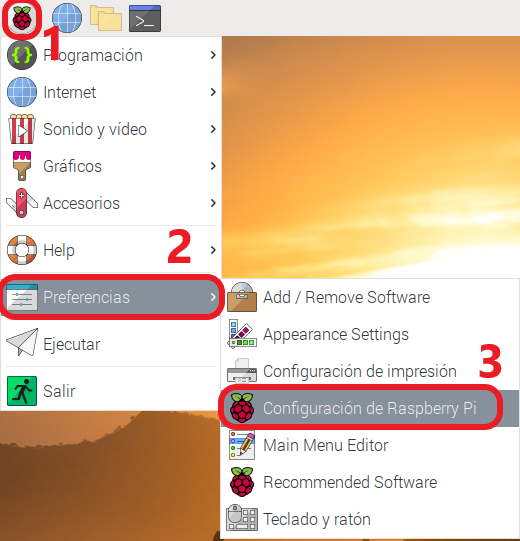
\includegraphics[width=0.8\textwidth]{img/Instalación/tempsnip.png}
\caption{Configura VNC 1.}\label{VNC1}
\end{figure}

Cuando abra la ventana, debemos acceder a la pestaña <<interfaces>> y activar VNC como podemos ver en la imagen~\ref{VNC2}:

\begin{figure}[h]
\centering
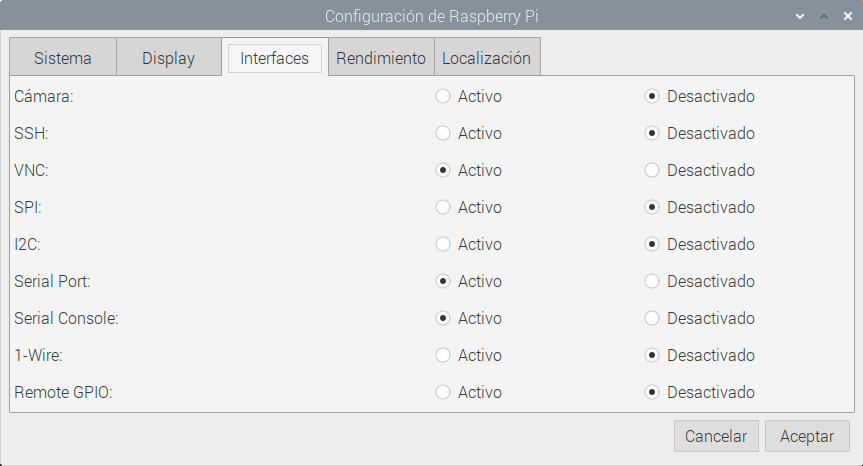
\includegraphics[width=0.8\textwidth]{img/Instalación/vnc2.PNG}
\caption{Configura VNC 2.}\label{VNC2}
\end{figure}

De esta forma podemos acceder desde VNC Viewer a nuestra máquina sabiendo la dirección IP, usuario y contraseña de ésta.

\subsection{Descarga e instalación del software SDI}
Para descargarnos e instalar el software SDI debemos seguir los siguientes pasos:

\begin{enumerate}
    \item Descargar la última release que exista en el repositorio de GitHub en el formato que se prefiera:~\url{https://github.com/davidelinformatico/TFG/releases}
    \item Para extraer del archivo .tar utilizar:~\\ \texttt{tar -xvf SistemaDomoticoInteligente\_v1.0.tar}.
    \item Para extraer del archivo .tar.gz utilizar:~\\ \texttt{tar xzvf SistemaDomoticoInteligente\_v1.0.tar.gz}.
\end{enumerate}
En este punto ya tendremos todos los archivos extraídos.

El siguiente paso es rellenar el archivo \texttt{config2.bot} con los tokens obtenidos anteriormente y la información de estancias donde se sitúan los periféricos y sus pines de control.

Ahora instalaremos el software. Para ello accederemos a \textbf{\textasciitilde/source/scripts/auto/} y corremos el archivo \texttt{setup.sh} con la siguiente sentencia:
\begin{lstlisting}[language=sh,firstnumber=0]
sh setup.sh
\end{lstlisting}

En este momento se descargarán todos los elementos necesarios de internet y se instalarán.

\subsection{Automatizado y puesta a producción}
Uno de los puntos de la automatización es la generación de un demonio para nuestro bot de forma que se ejecutará con el inicio del sistema y podremos trabajar con el una sencilla sentencia:

\begin{lstlisting}[language=sh,firstnumber=0]
sudo systemctl bot stop
\end{lstlisting}
\begin{lstlisting}[language=sh]
sudo systemctl bot start 
\end{lstlisting}
Para conseguirlo, he realizado los siguientes pasos:

Se debe generar el archivo de nuestro demonio en lib/systemd/system/ con la extensión <<.service>>:
\begin{lstlisting}[language=sh, firstnumber=0]
sudo nano /lib/systemd/system/bot.service
\end{lstlisting}
El contenido del archivo es:
\begin{lstlisting}[language=sh, caption={Modificaciones en el archivo /lib/systemd/system/bot.service.}, firstnumber=0]
[Unit]
Description=Lanza el bot de control domotico
After=network.target
StartLimitIntervalSec=0

[Service]
Type=simple
Restart=always
RestartSec=1
User=pi
WorkingDirectory=/home/pi/source/TFG/scripts/bot/
ExecStart=/usr/bin/env python3 /home/pi/source/TFG/scripts/bot/bot.py

[Install]
WantedBy=multi-user.target
\end{lstlisting}
Después debemos actualizar los demonios con: 
\begin{lstlisting}[language=sh, firstnumber=0]
systemctl daemon-reload
\end{lstlisting}
Iniciar el demonio: 
\begin{lstlisting}[language=sh, firstnumber=0]
sudo systemctl start bot
\end{lstlisting}
Parar el demonio: 
\begin{lstlisting}[language=sh, firstnumber=0]
sudo systemctl stop bot
\end{lstlisting}
Estado del demonio, con el que podremos conocer el pid~\footnote{Identificador del proceso}, que siempre es útil: 
\begin{lstlisting}[language=sh, firstnumber=0]
sudo systemctl status bot
\end{lstlisting}

Para incluirlo en el inicio de la máquina habría que moverlo a /etc/init.d y luego ejecutar: 
\begin{lstlisting}[language=sh, firstnumber=0]    
sudo update-rc.d bot defaults
sudo systemctl daemon-reload
sudo systemctl enable bot
sudo systemctl start bot
\end{lstlisting}  

Con esto tendríamos el software completamente instalado.

\section{Inclusión de usuarios en el bot}
El primer paso es buscar el bot por su nombre. En mi caso se llama \textbf{SDI\_Domo\_bot}.
Una vez localizado, accedemos a él y le enviamos un mensaje. A lo que nuestro bot nos responderá con un mensaje con un número largo. Éste número largo es el que debemos incluir en el apartado de usuarios dentro del archivo config2.bot.

